% !TEX program = xelatex
\documentclass{article}
\usepackage{/Users/Jay/LaTeX/cs}
\usepackage{/Users/Jay/LaTeX/codelist}
\usepackage{/Users/Jay/LaTeX/xeCJK}

\newcommand{\hmwkClass}{Virtual Reality, Spring 2018}
\newcommand{\hmwkTitle}{Final Project Report}
\newcommand{\hmwkDueDate}{June 26, 2018}
\newcommand{\tb}{\textbf}

\begin{document}

\thispagestyle{empty}
\section*{\hmwkClass \\
    \normalsize{\hmwkTitle} \\
    \normalsize{DUE DATE: \hmwkDueDate}
}

\hfill{B03902129 \, 資工四 \, 陳鵬宇} \\

\section*{MonsterGo}

A VR game built with Unity. And I've put all source code in the GitHub site: https://github.com/walkccc/MonsterGo

\section*{Getting Started}

I use Unity to build this project.

To keep things as tiny as possible, I didn't include all files in this repo, but you can still build them step by step.

After cloning this repo, open the project with Unity. It'll import some necessary files.

Then navigate to Assets/DataFiles/Scenes, you can preview the game with different scenes here.

\section*{Dependencies}

The setup in my computer:

\begin{lstlisting}
Unity Hub                               Version 0.17.1
Unity                                   Version 2018.1.3f1 Personal
GVR SDK for Unity v1.130.1              GoogleVRForUnity_1.130.1.unitypackage
macOS High Sierra                       Version 10.13.5
Xcode                                   Version 9.3 (9E145)
\end{lstlisting}

\section*{Build Settings}

After cloning this repo, select File > Build Settings in the top bar.

Then choose the Platform you want to run and press Switch Platform. It'll take some time to import the assets. Here I use iOS as example.

Also, make sure that the order of \tb{Scenes In Build} in the Build Settings as follows:

\begin{lstlisting}
DataFiles/Scenes/MainScene              0
DataFiles/Scenes/DayScene               1
DataFiles/Scenes/NightScene             2
DataFiles/Scenes/EndScene               3
\end{lstlisting}

Then click the Player Settings.

In Settings for iOS -> Orientation -> Default Orientation*, select Landscape Left.

Otherwise, it'll cause unexpected behavior in your iPhone! (I haven't tested the behavior on Android Platform.)

\section*{Running the app}

In the top bar, select Build \& Run and press the Build And Run button in the bottom right, then save the project to any name you want.

Unity will then open the Xcode automatically, and make sure to choose the Team option (Here I choose Personal Team) in the Signing field.

Have fun with the MonsterGo!

\section*{Scripts Description}

There are four scenes in default:

\begin{itemize}
    \item MainScene: main menu
    \item DayScene: day mode
    \item NightScene: night mode
    \item EndScene: end menu
\end{itemize}

\begin{lstlisting}
    public void LoadDayScene () {
		SceneManager.LoadScene ("DayScene");
	}

	public void LoadNightScene () {
		SceneManager.LoadScene ("NightScene");
	}

	public void QuitGame () {
		Application.Quit ();
		Debug.Log ("Quit Game!");
	}
\end{lstlisting}

In the game, you have to throw PockBall to catch the monsters, thus I maintain the number of monsters catched in order to display the final score in the EndScene.

\begin{lstlisting}
public class Mcalculator : MonoBehaviour {

	public int counter;
	public TextMesh totalMonster;

	void Start () {
		counter = 0;
		DontDestroyOnLoad (gameObject);
    }

	public void totalCount () {
		counter = counter + 1;
		totalMonster.text = counter.ToString ();
		Debug.Log ("Monsters Collected: " + counter);
	}
}
\end{lstlisting}

I also give each monster a tag to identify which monster we trigger, and each time OnTriggerEnter() is invoked, i.e., the PokeBall hit a monster, it should call mcalc.totalCount() to add 1.

\begin{lstlisting}
    public class MonstersCollected : MonoBehaviour {

        Mcalculator mcalc;
    
        void Start () {
            mcalc = FindObjectOfType<Mcalculator> ();
        }
        
        public void OnTriggerEnter (Collider collide) {
            if (collide.gameObject.CompareTag ("GhostGreen") ||
                collide.gameObject.CompareTag ("GhostViolet") ||
                collide.gameObject.CompareTag ("RabbitRed") ||
                collide.gameObject.CompareTag ("RabbitYellow") ||
                collide.gameObject.CompareTag ("SlimeBlue") ||
                collide.gameObject.CompareTag ("SlimeRed")) {
                Destroy (collide.gameObject);
                Destroy (gameObject);
                mcalc.totalCount ();
            }
        }
    
        void OnCollisionEnter(Collision col) {
            if (col.gameObject.CompareTag ("ground")) {
                Destroy (gameObject);
            }
        }
    }
\end{lstlisting}

To generate the environment and monsters, I use random function to quick build it:

\begin{lstlisting}
public class RandomEnvs : MonoBehaviour {

	public GameObject [] diffTreeRocks;
	public GameObject [] diffGrassRocks;

	void Start () {
		for (int i = 0; i < Random.Range (600, 700); i++) {
			TreeRockCount ();
		}

		for (int j = 0; j < Random.Range (1000, 1200); j++) {
			GrassRockCount ();
		}
	}

	void TreeRockCount () {
		int treeRockIdx = Random.Range (0, diffTreeRocks.Length);
		GameObject randomTreeRock = Instantiate (diffTreeRocks [treeRockIdx]);
		randomTreeRock.transform.parent = transform;
		randomTreeRock.transform.localPosition = new Vector3(Random.Range (-95, 95), 0.0f, Random.Range (-95, 95));
	}

	void GrassRockCount () {
		int grassRockIdx = Random.Range (0, diffGrassRocks.Length);
		GameObject randomGrassRock = Instantiate (diffGrassRocks [grassRockIdx]);
		randomGrassRock.transform.parent = transform;
		randomGrassRock.transform.localPosition = new Vector3(Random.Range (-95, 95), 0.0f, Random.Range (-95, 95));
	}
}

public class RandomMonsters : MonoBehaviour {

	public GameObject [] diffMonsters;

	void Start () {
		for (int i = 0; i < Random.Range (800, 900); i++) {
			MonsterCount ();
		}
	}

	void MonsterCount () {
		int index = Random.Range (0, diffMonsters.Length);
		GameObject randomMonster = Instantiate (diffMonsters [index]);
		randomMonster.transform.parent = transform;
		randomMonster.transform.localPosition = new Vector3(Random.Range (-95, 95), 0.0f, Random.Range (-95, 95));
	}
}
\end{lstlisting}

Finally, it is important to specify the moving behavior, thus making it easy to play in VR environment. I let the player walking in the speed of deltaTime * speed (this can be any number).

\begin{lstlisting}
public class WalkandShoot : MonoBehaviour {

	public GameObject pokeball;
	public float shootingSpeed = 10;
	public float speed;

	void Update () {
		transform.position = transform.position + Camera.main.transform.forward * speed * Time.deltaTime;

		if (Input.GetButtonDown ("Fire1")) {
			GameObject pokego = Instantiate (pokeball);
			pokego.transform.position = transform.position;
			Rigidbody rb = pokego.GetComponent<Rigidbody> ();
			Camera cam = GetComponentInChildren<Camera> ();
			rb.velocity = cam.transform.rotation * Vector3.forward * shootingSpeed;
		}
	}
}
\end{lstlisting}

\section*{Screenshots}

\begin{figure}[!htb]
    \centering
    \begin{subfigure}[b]{0.49\textwidth}
        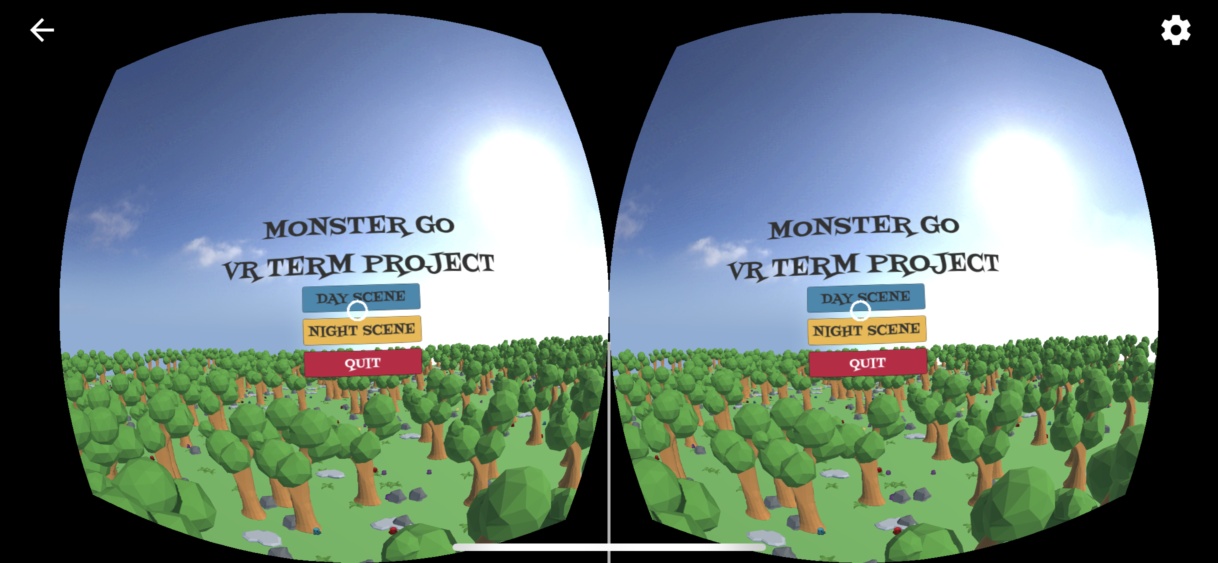
\includegraphics[width=\textwidth]{Screenshots/MainScene.png}
        \caption{MainScene}
    \end{subfigure}
    ~
    \begin{subfigure}[b]{0.49\textwidth}
        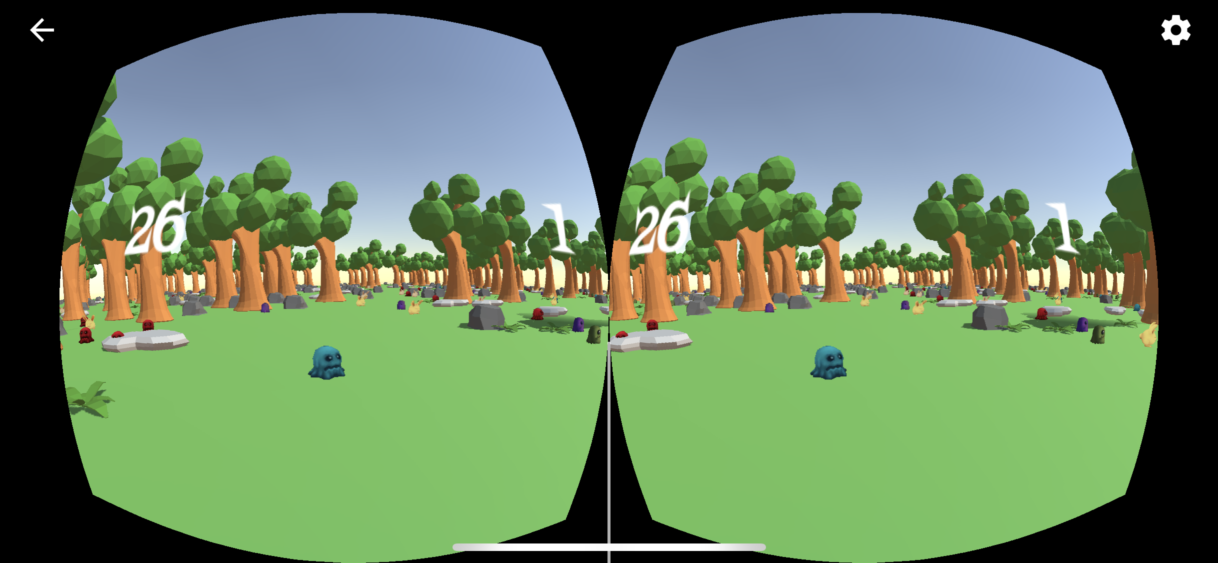
\includegraphics[width=\textwidth]{Screenshots/DayScene.png}
        \caption{DayScene}
    \end{subfigure}
    ~
    \begin{subfigure}[b]{0.49\textwidth}
        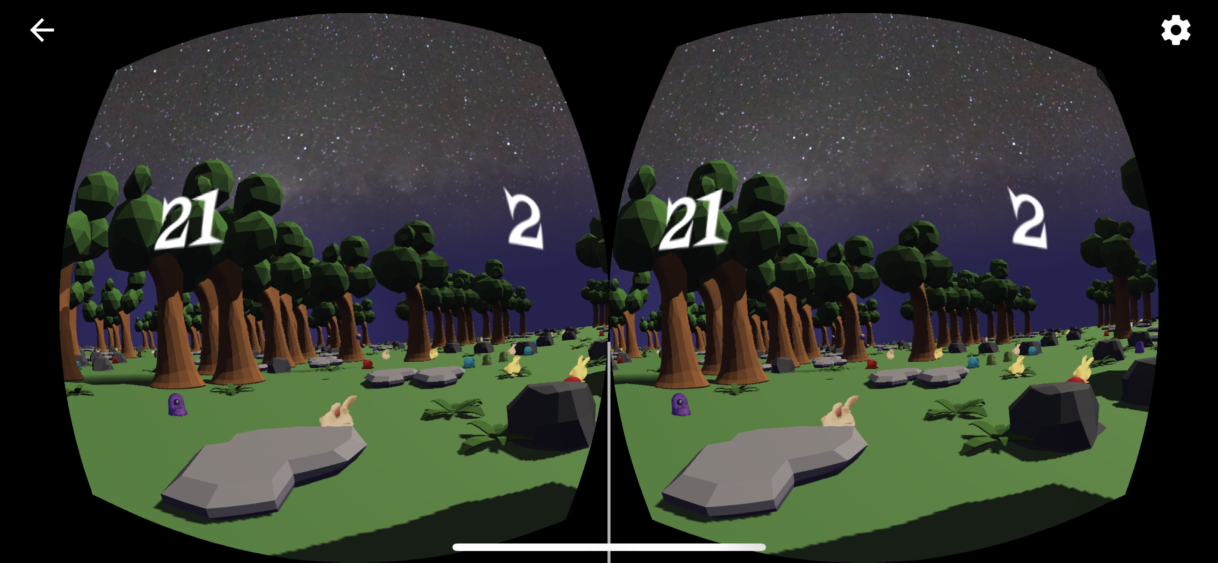
\includegraphics[width=\textwidth]{Screenshots/NightScene.png}
        \caption{NightScene}
    \end{subfigure}
    ~
    \begin{subfigure}[b]{0.49\textwidth}
        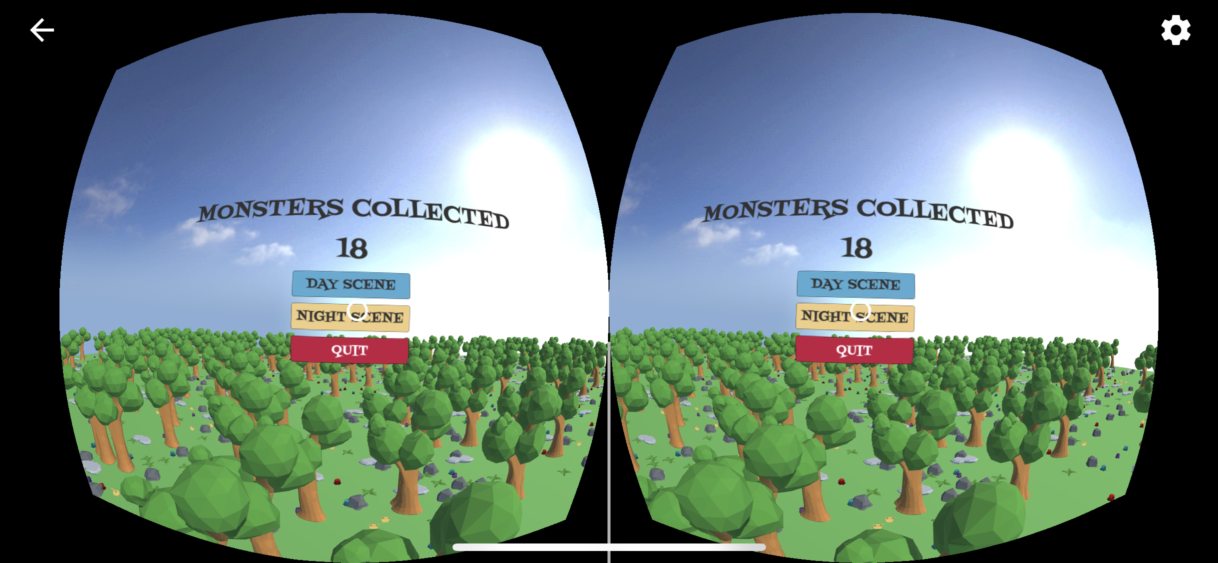
\includegraphics[width=\textwidth]{Screenshots/EndScene.png}
        \caption{EndScene}
    \end{subfigure}
\end{figure}

\section*{Conclusion}

I'm happy to build this project and I also learned a lot of skill to write C\# codes this time. Building a VR environment and playing the VR game self-written is really interesting! I've also review some basic physics knowledge since I have to specify the moving behavior correctly and choose the right parameters. However, even in a small mobile game, motion sickness still happened. It's pity to face this situation, but I think in the future the technology of VR will become much more mature.

\end{document}